
The most extreme corruptions mentioned in section \ref{section:nuclei-preprocessing} were removed, yet some of the images that are corrupted not that severely (meaning they still have all the visible features needed for learning) were left in the dataset in order to not critically reduce the amount of data. The examples of these images are shown in Figure \ref{fig:lightning_conditions}.
\begin{figure}[H]
    \centering
    \setkeys{Gin}{width=\linewidth}
    \centering
        \begin{tabularx}{\textwidth}{YYYY}
            \textbf{Too few cells} &
            \textbf{Overexposure} &
            \textbf{Light gradient} &
            \textbf{Normal lightning} \\
            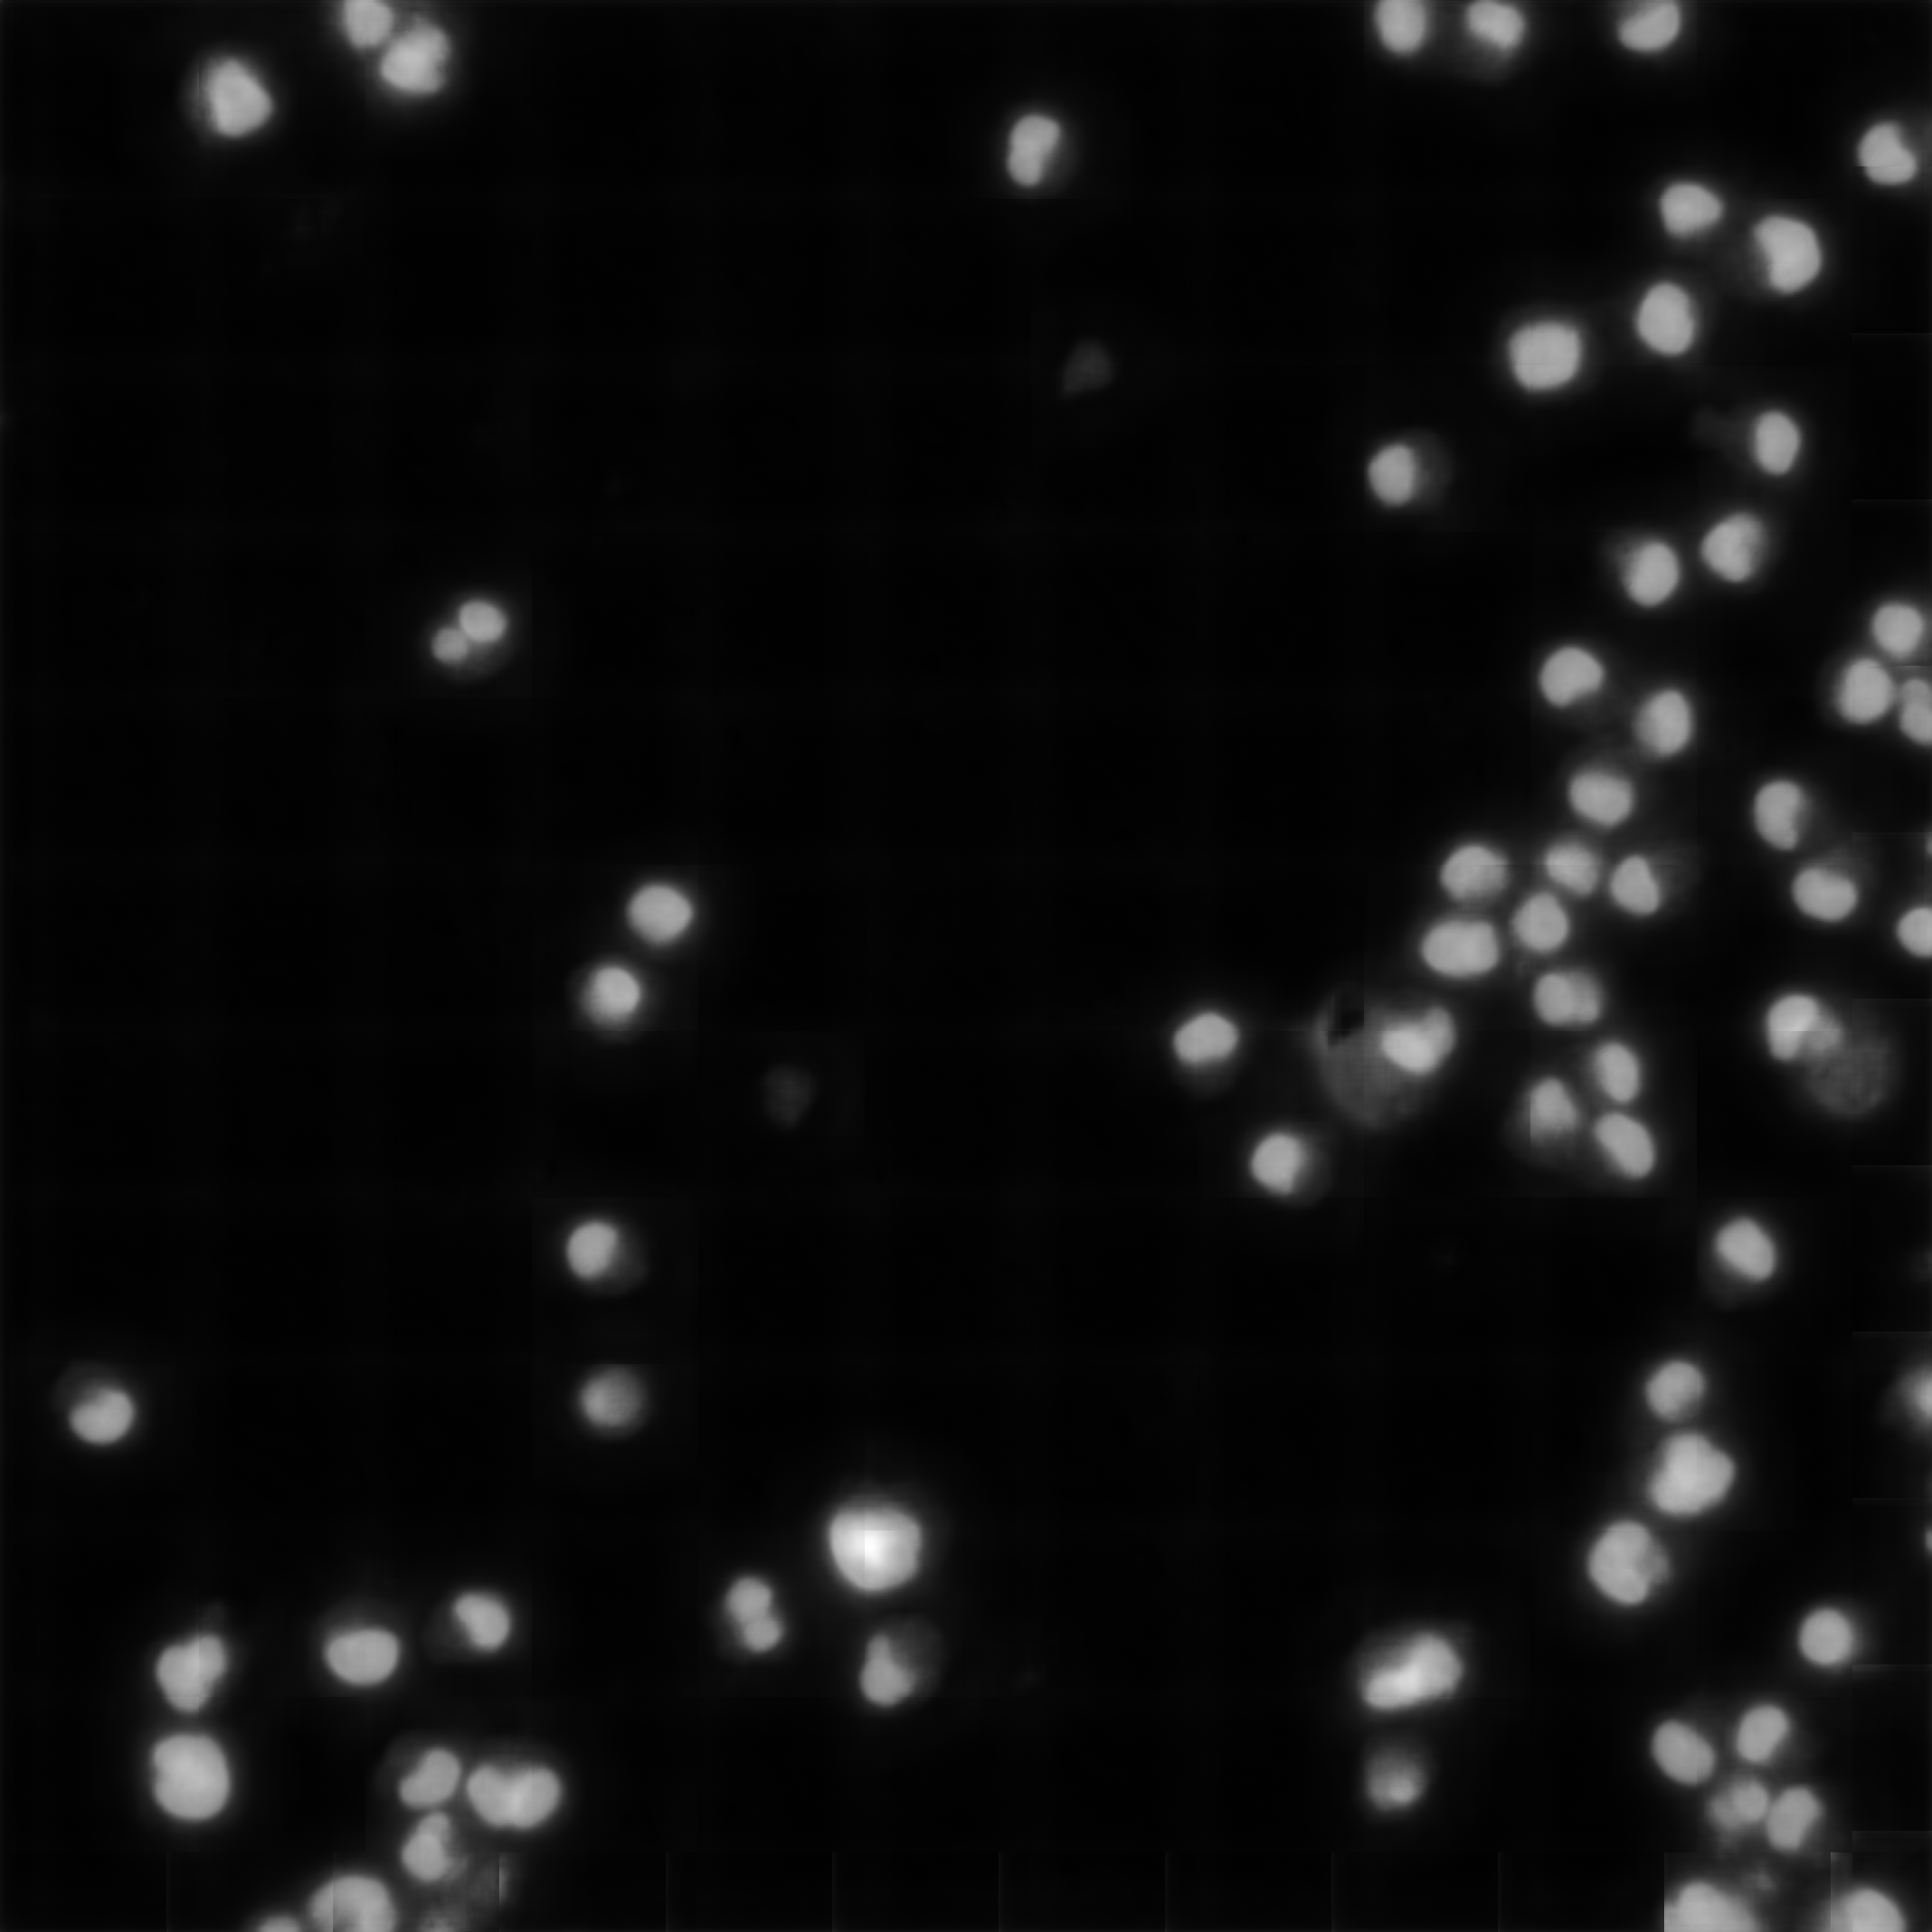
\includegraphics{bilder/lightning-conditions/lightning-1.png} & 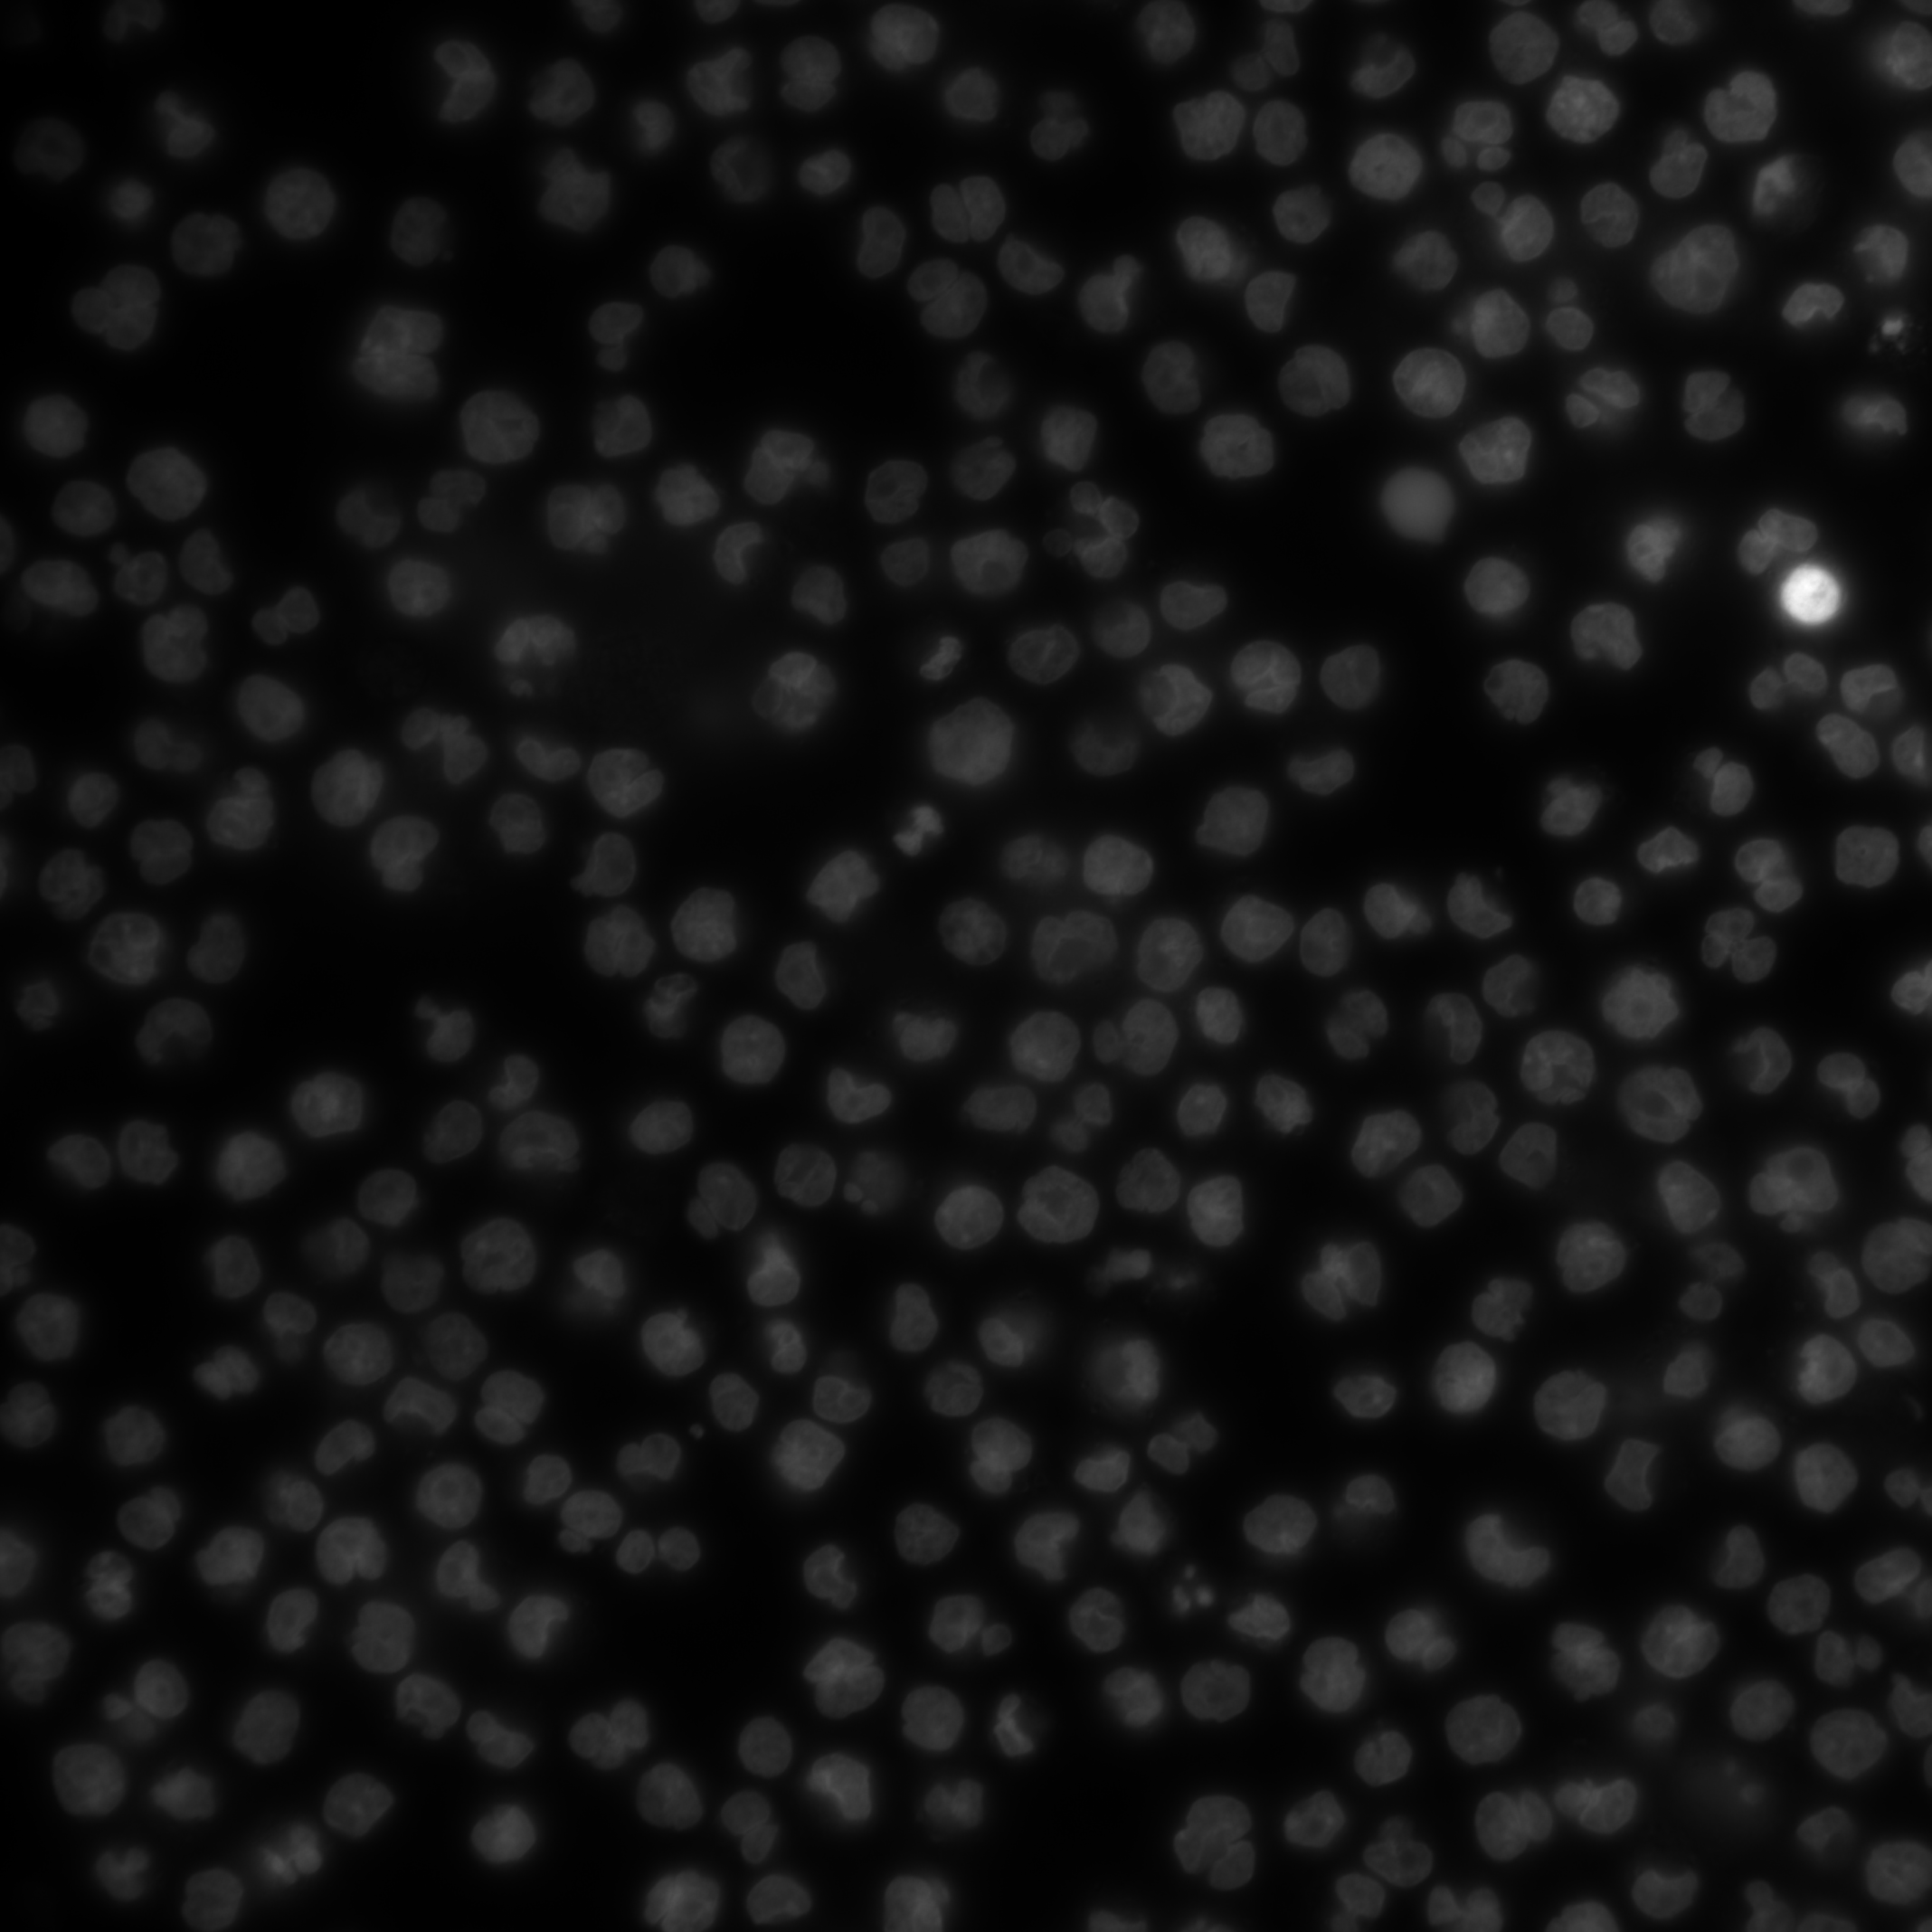
\includegraphics{bilder/lightning-conditions/lightning-2.png} &
            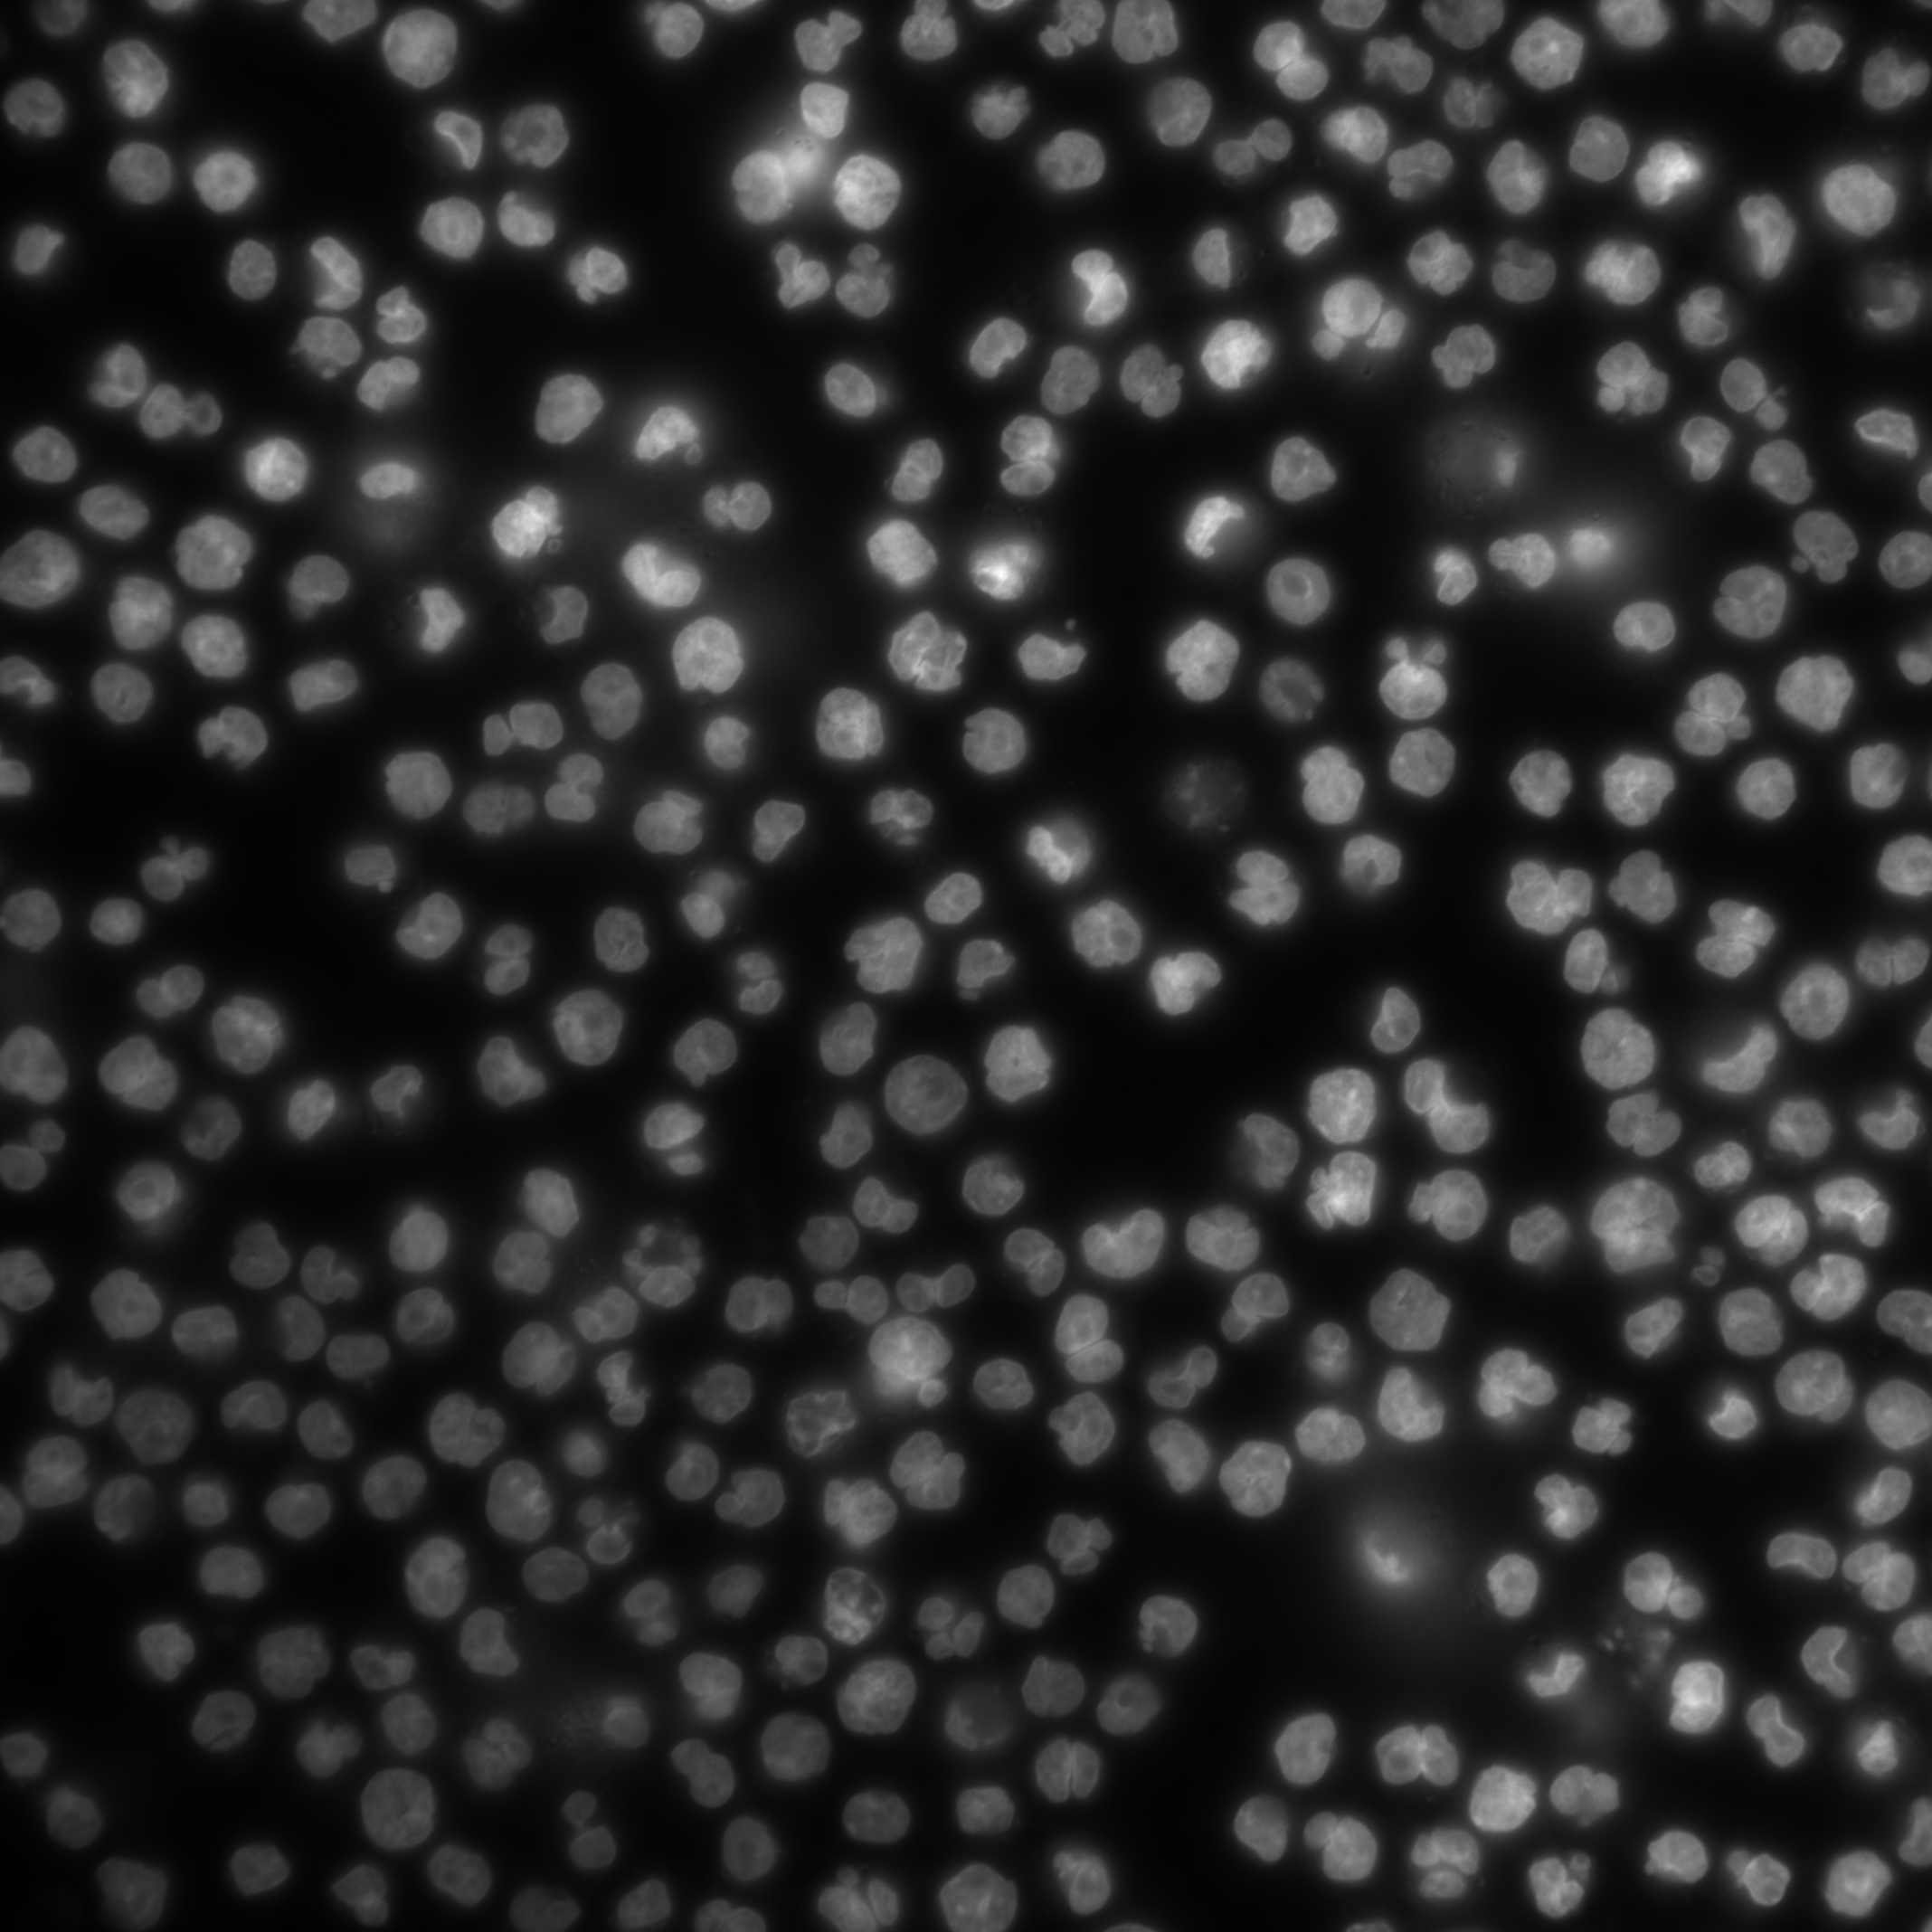
\includegraphics{bilder/lightning-conditions/lightning-3.png} & 
            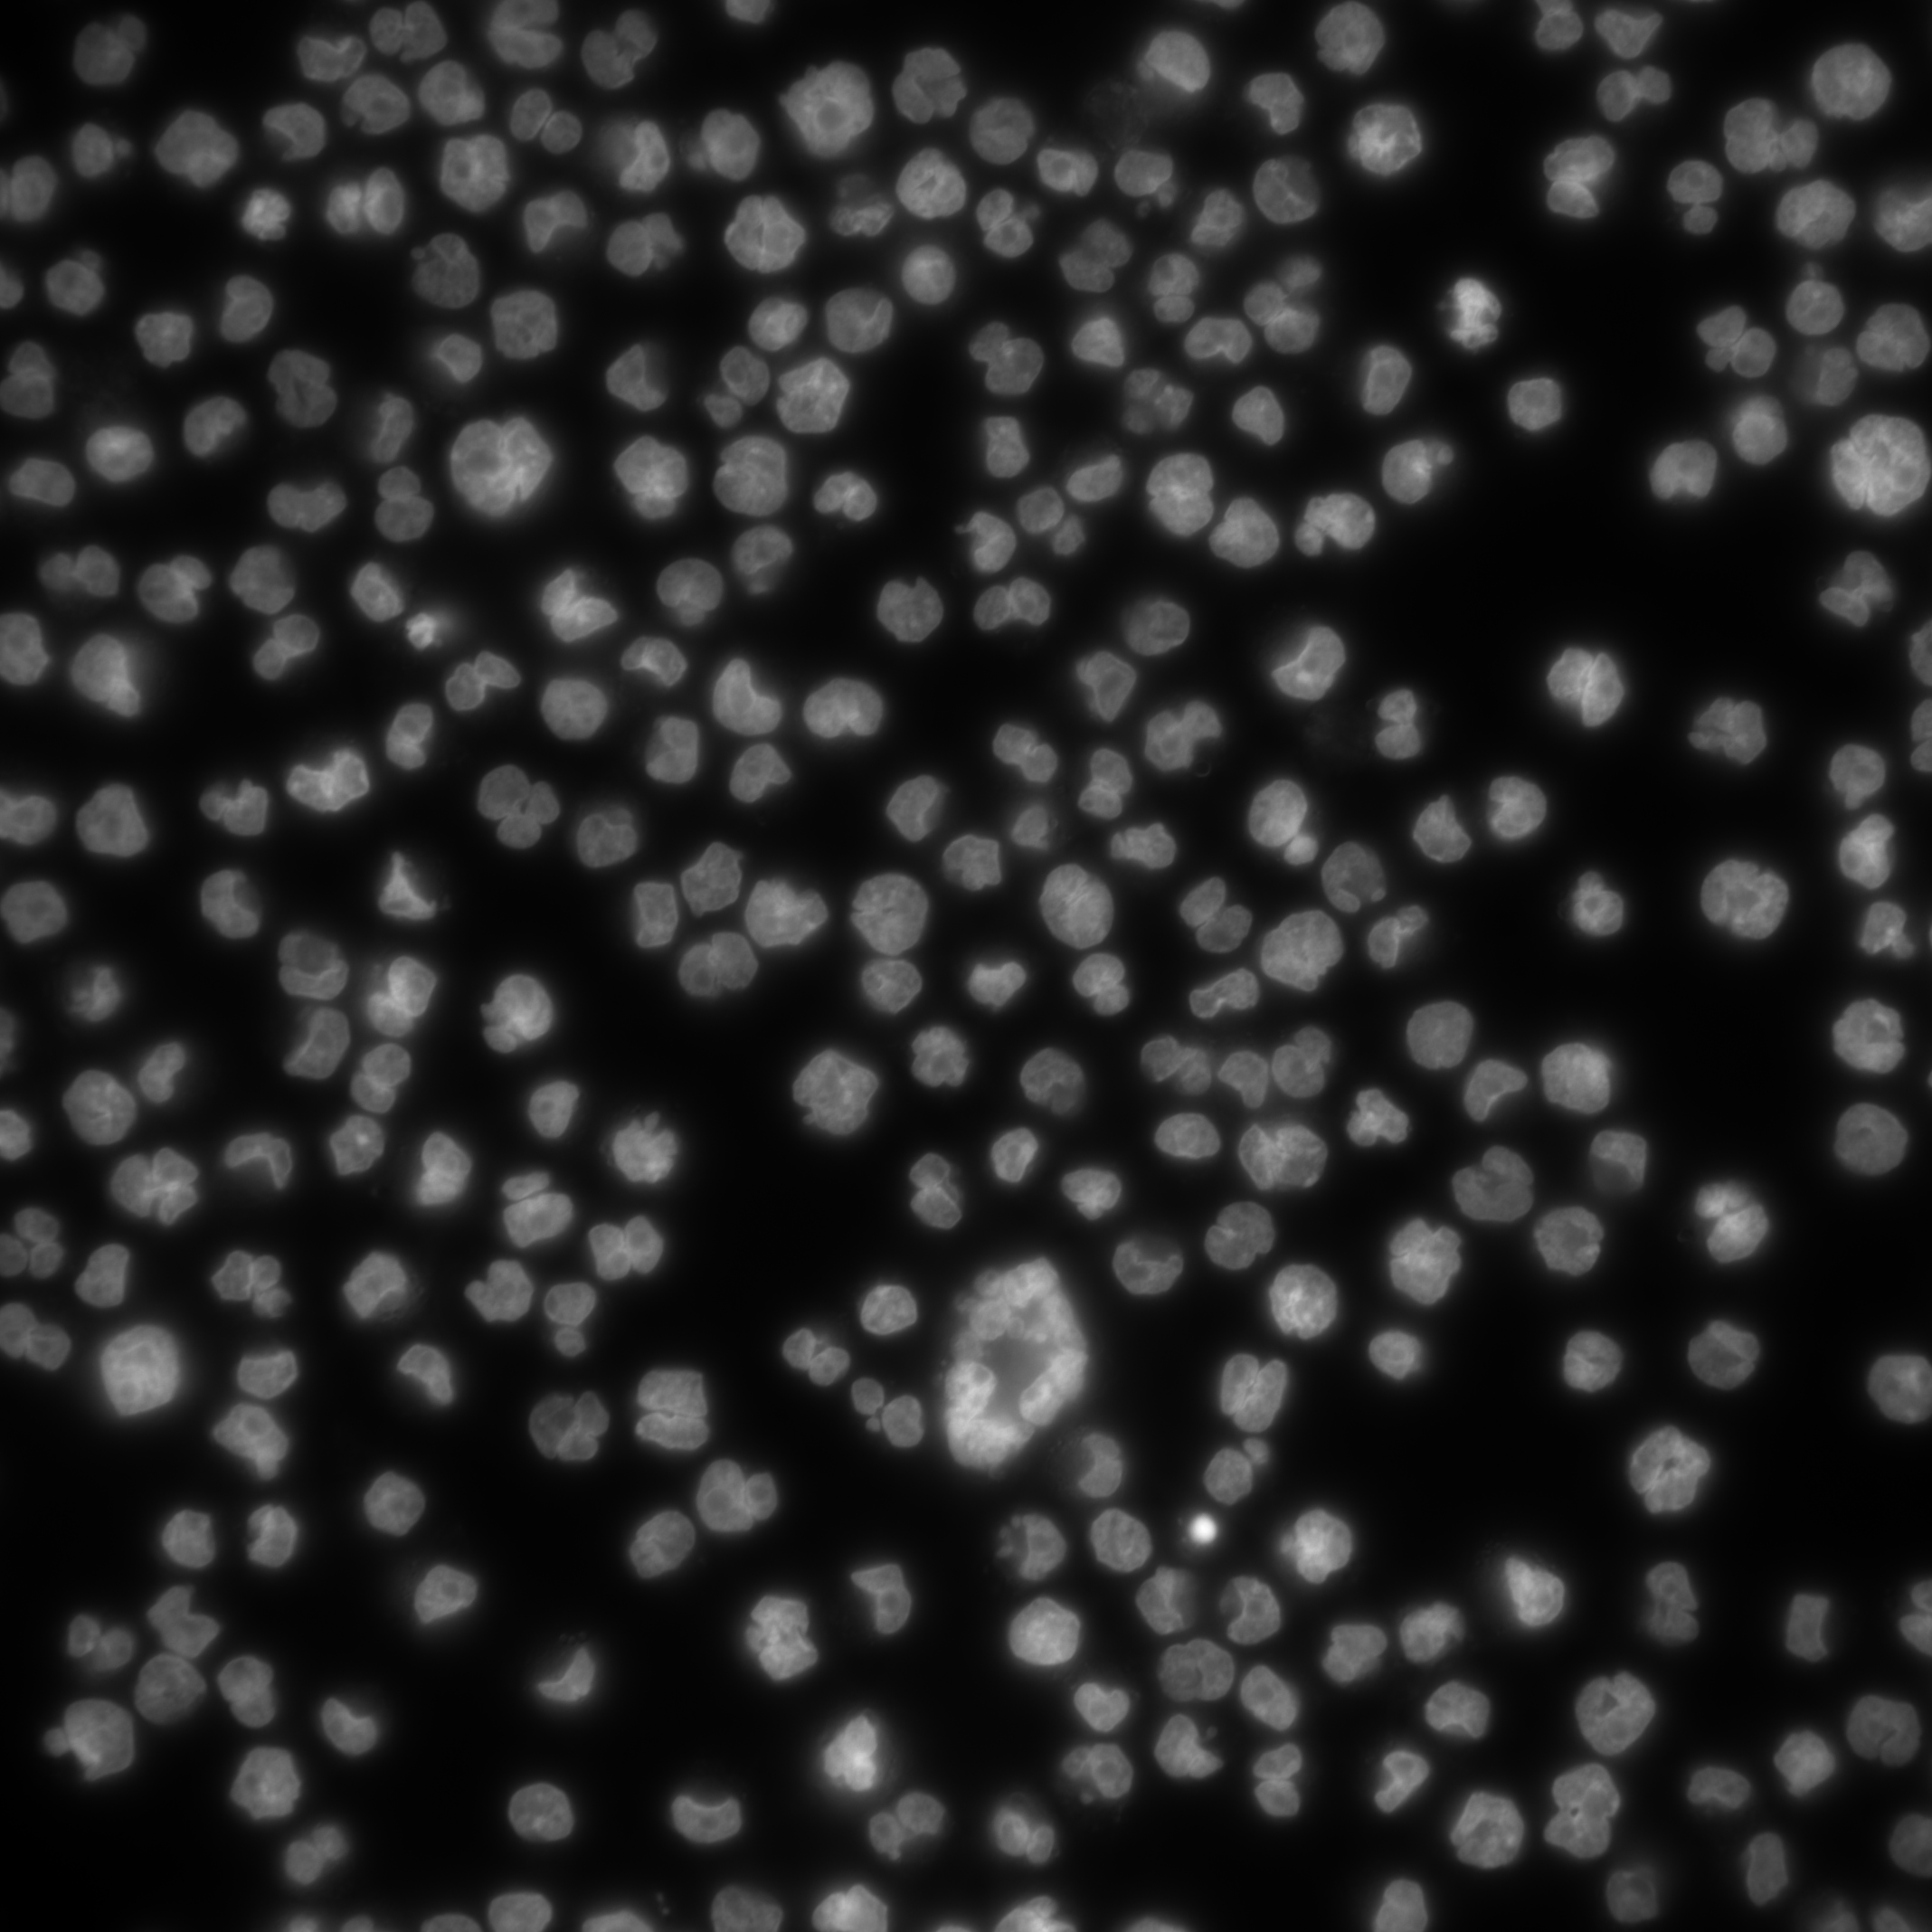
\includegraphics{bilder/lightning-conditions/lightning-4.png}
        \end{tabularx}
    \caption{Different lightning conditions}
    \label{fig:lightning_conditions}
\end{figure}

\begin{figure}[H]
    \centering
    \setkeys{Gin}{width=\linewidth}
    \centering
        \begin{tabularx}{\textwidth}{YY}
            \textbf{Original fluorescence} &
            \textbf{Segmentation} \\
            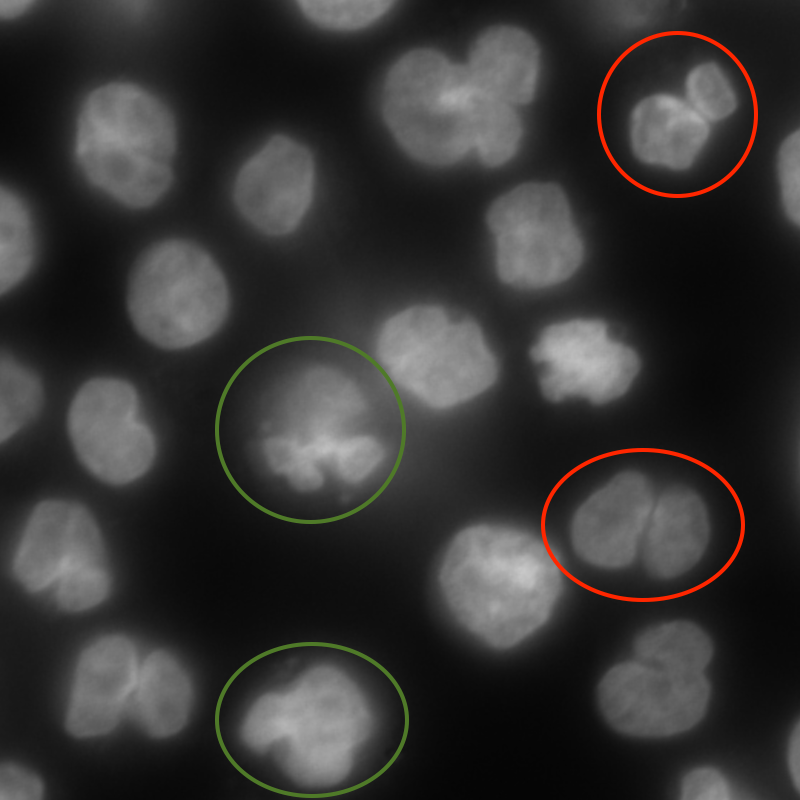
\includegraphics{bilder/close-located-cells/original.png} & 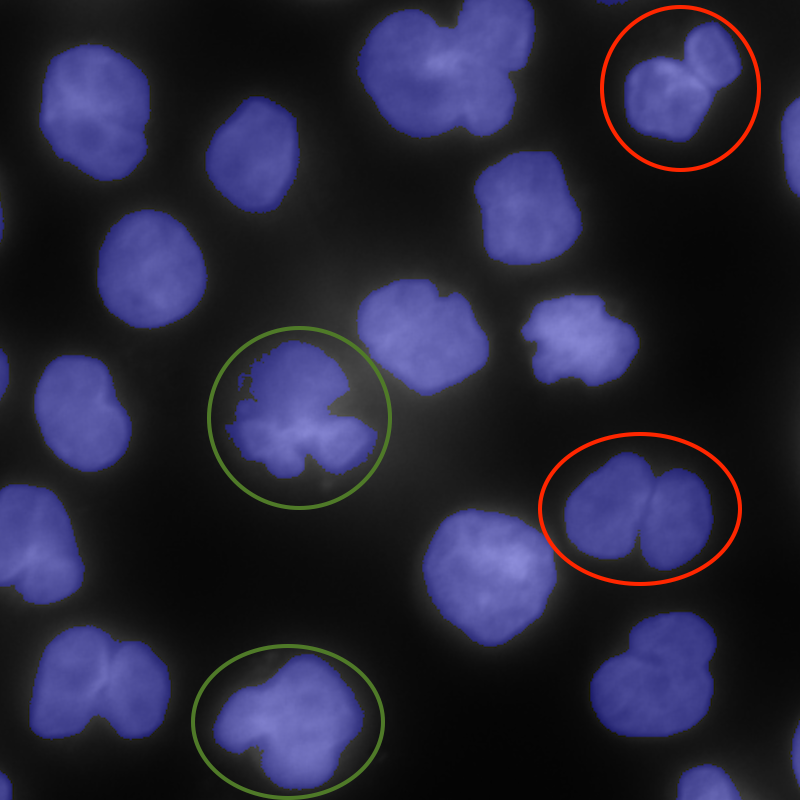
\includegraphics{bilder/close-located-cells/segmented.png}
        \end{tabularx}
    \caption{Closely located cells}
    \label{fig:closely-located-cells}
\end{figure}

Overall algorithm
\begin{figure}[H]
    \centering
    \setkeys{Gin}{width=\linewidth}
    \centering
        \begin{tabularx}{\textwidth}{YYYY}
            \textbf{Normalized input} &
            \textbf{Local threshold} &
            \textbf{Filled holes} &
            \textbf{Filtered regions} \\
            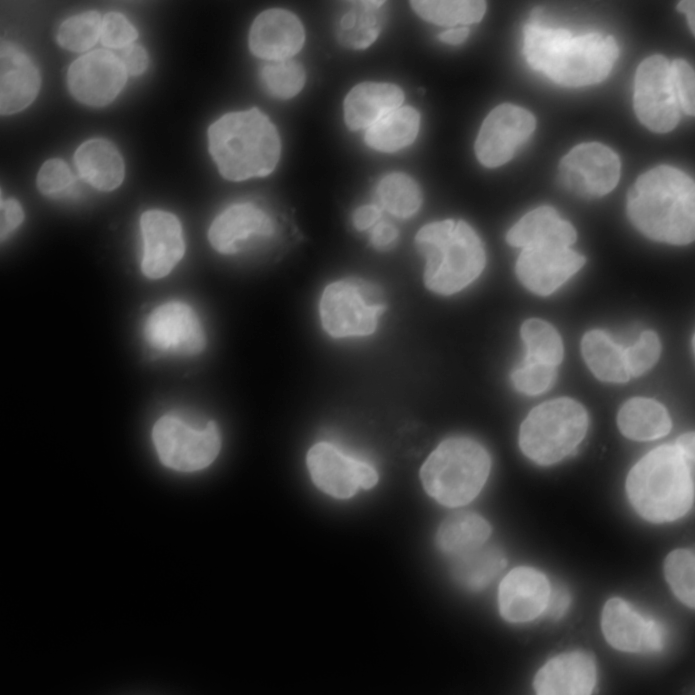
\includegraphics{bilder/segmentation/nuclei-mask/normalized.png} & 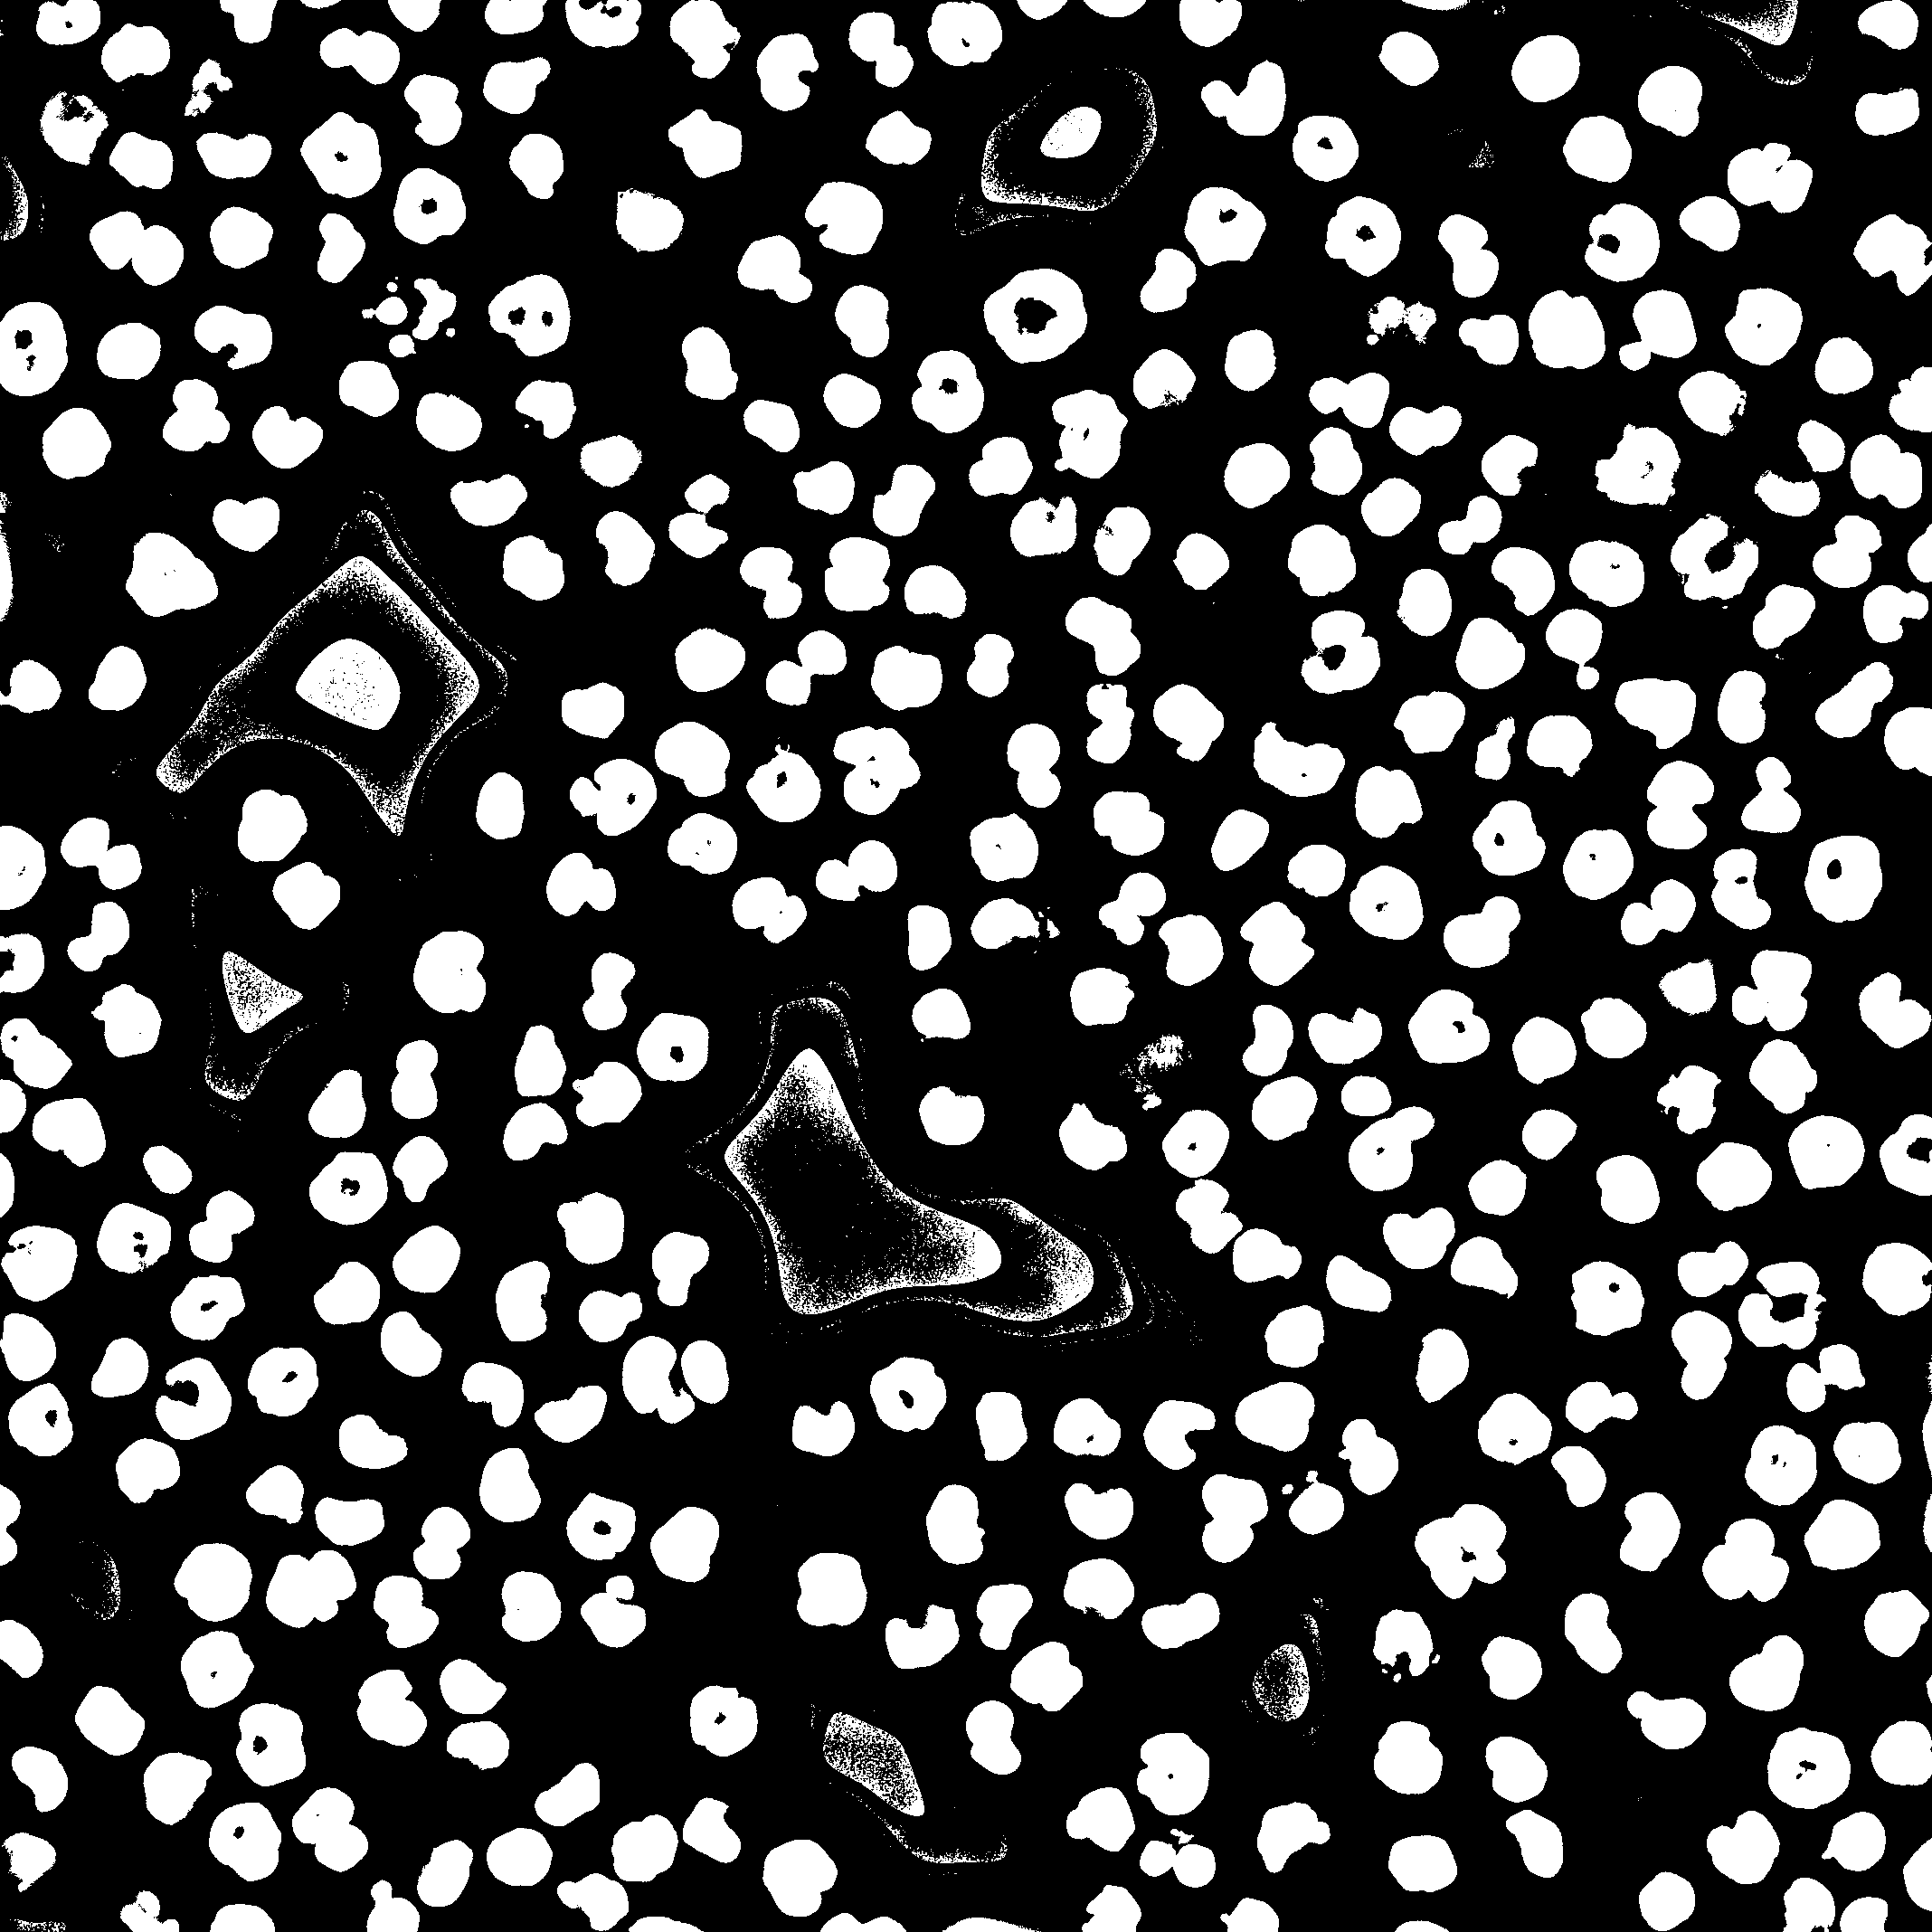
\includegraphics{bilder/segmentation/nuclei-mask/binary_local.png} &
            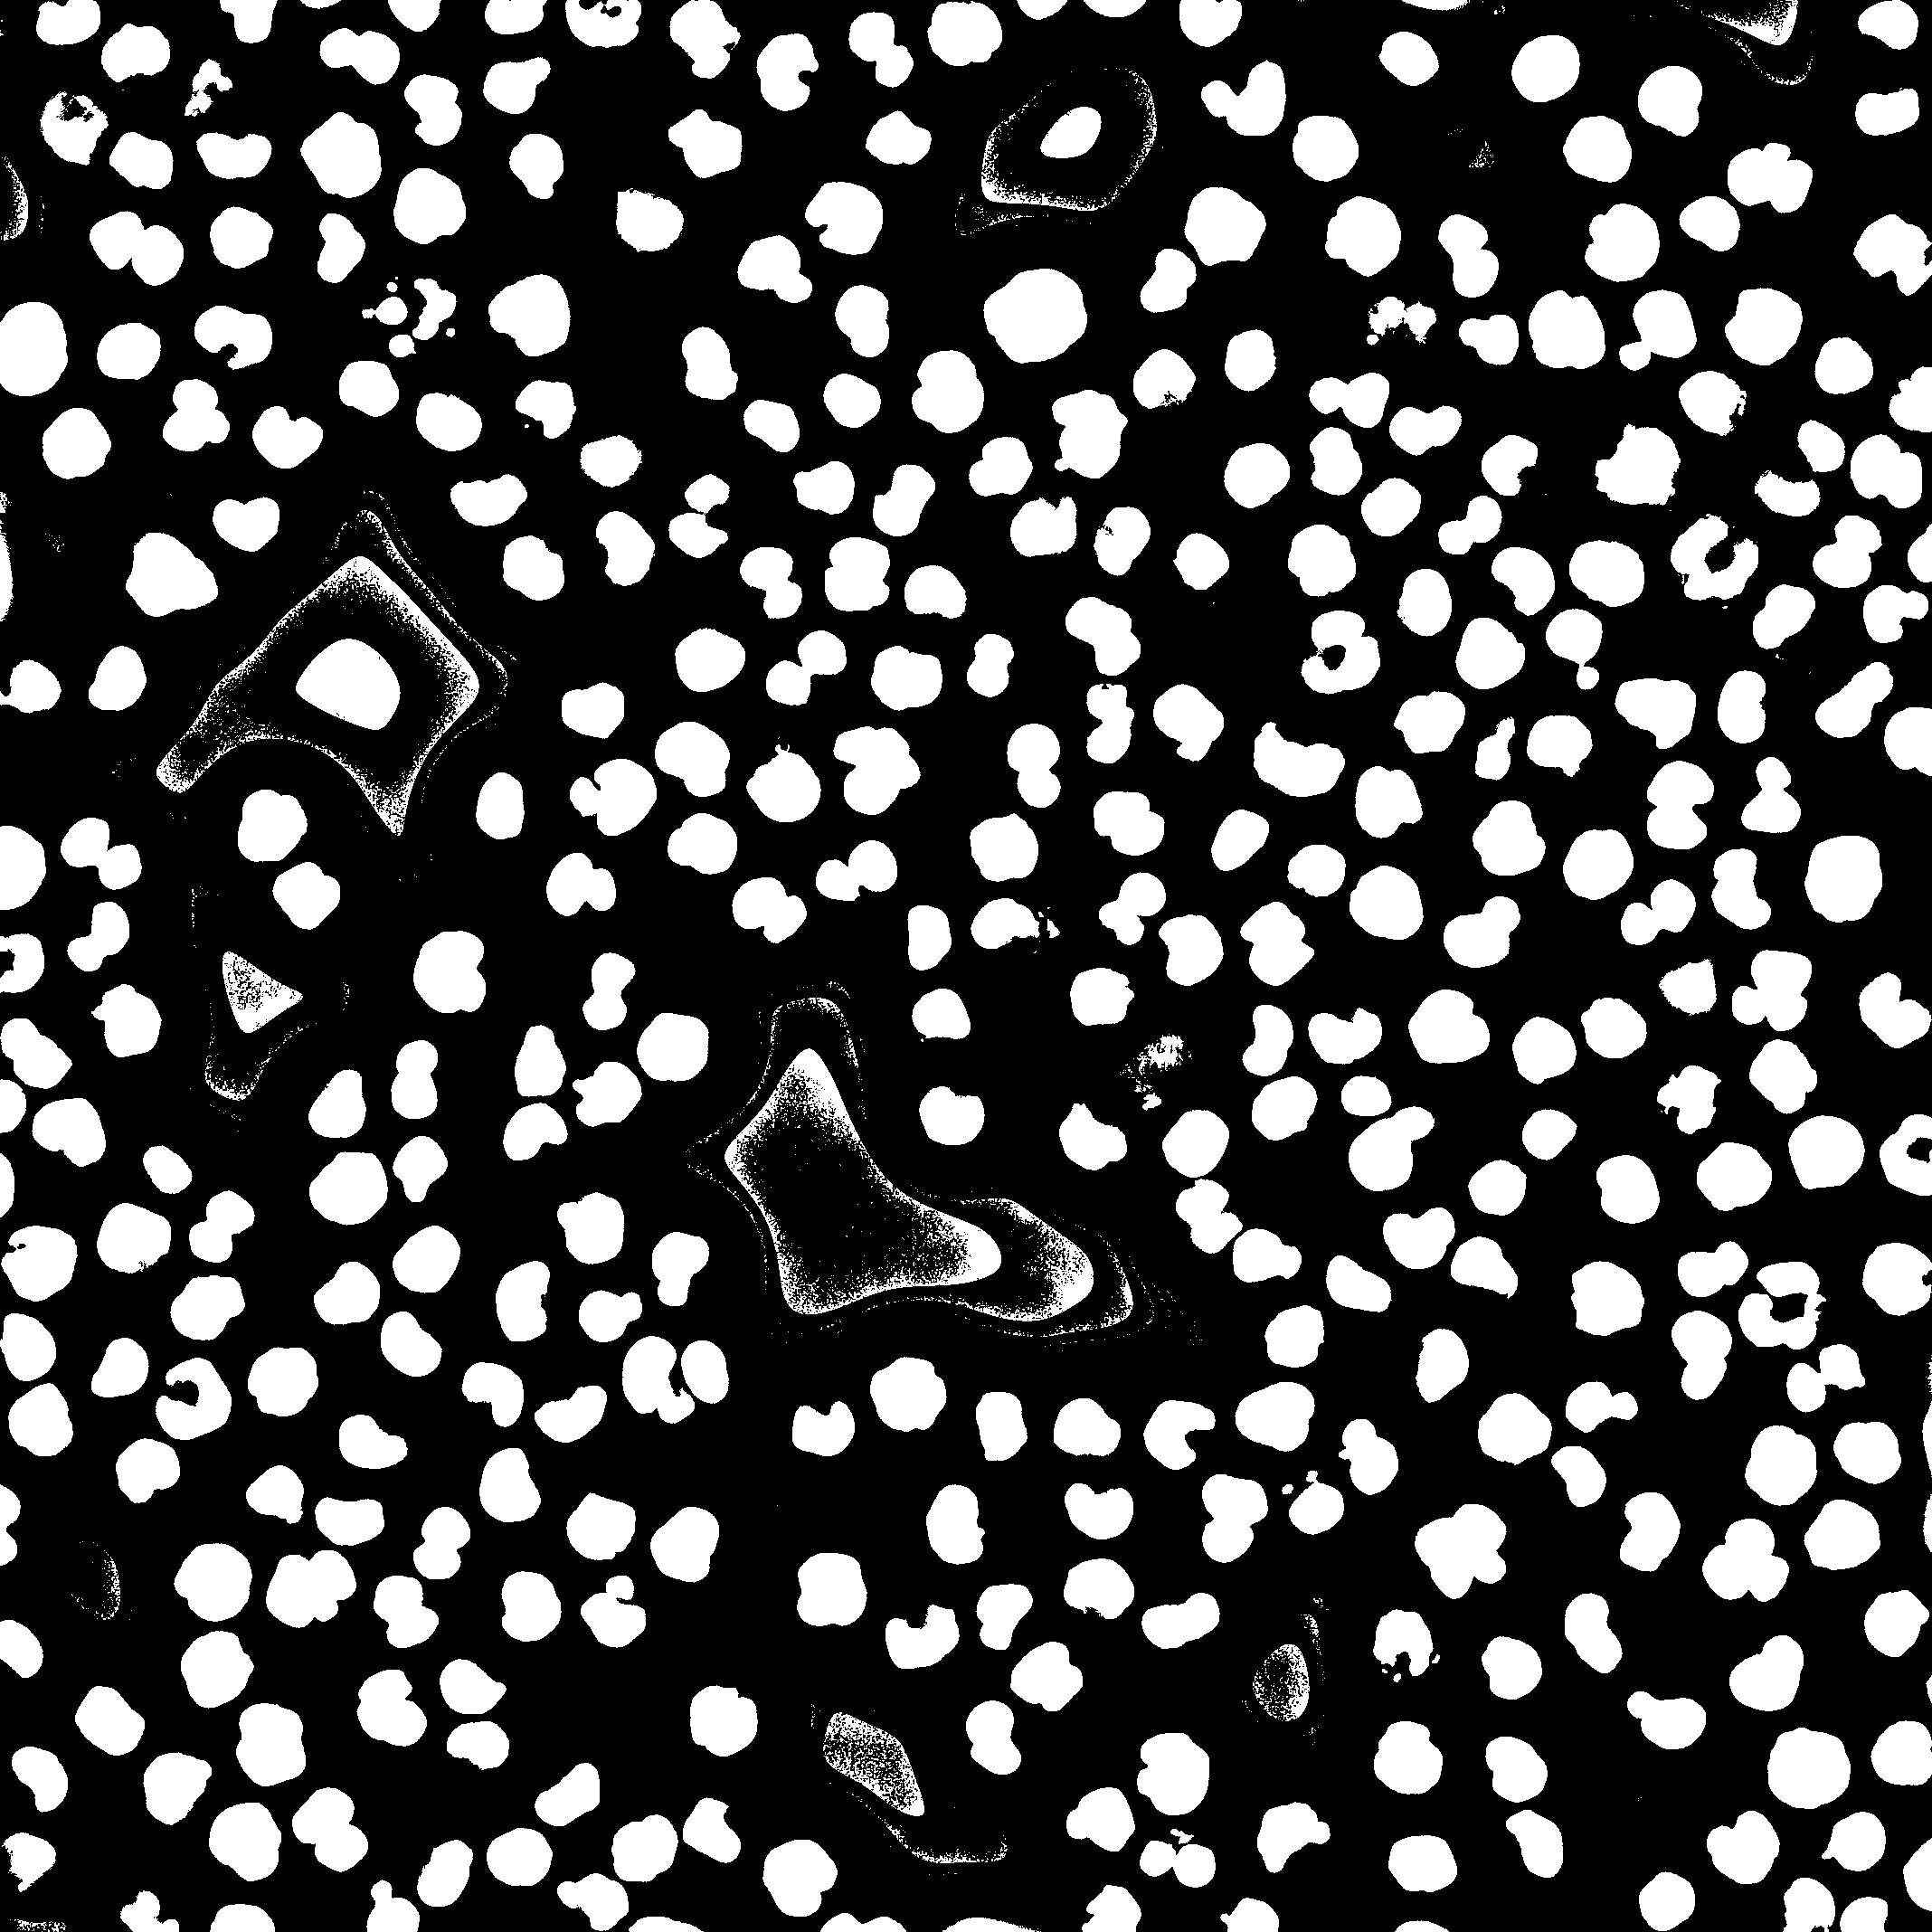
\includegraphics{bilder/segmentation/nuclei-mask/filled_holes.png} & 
            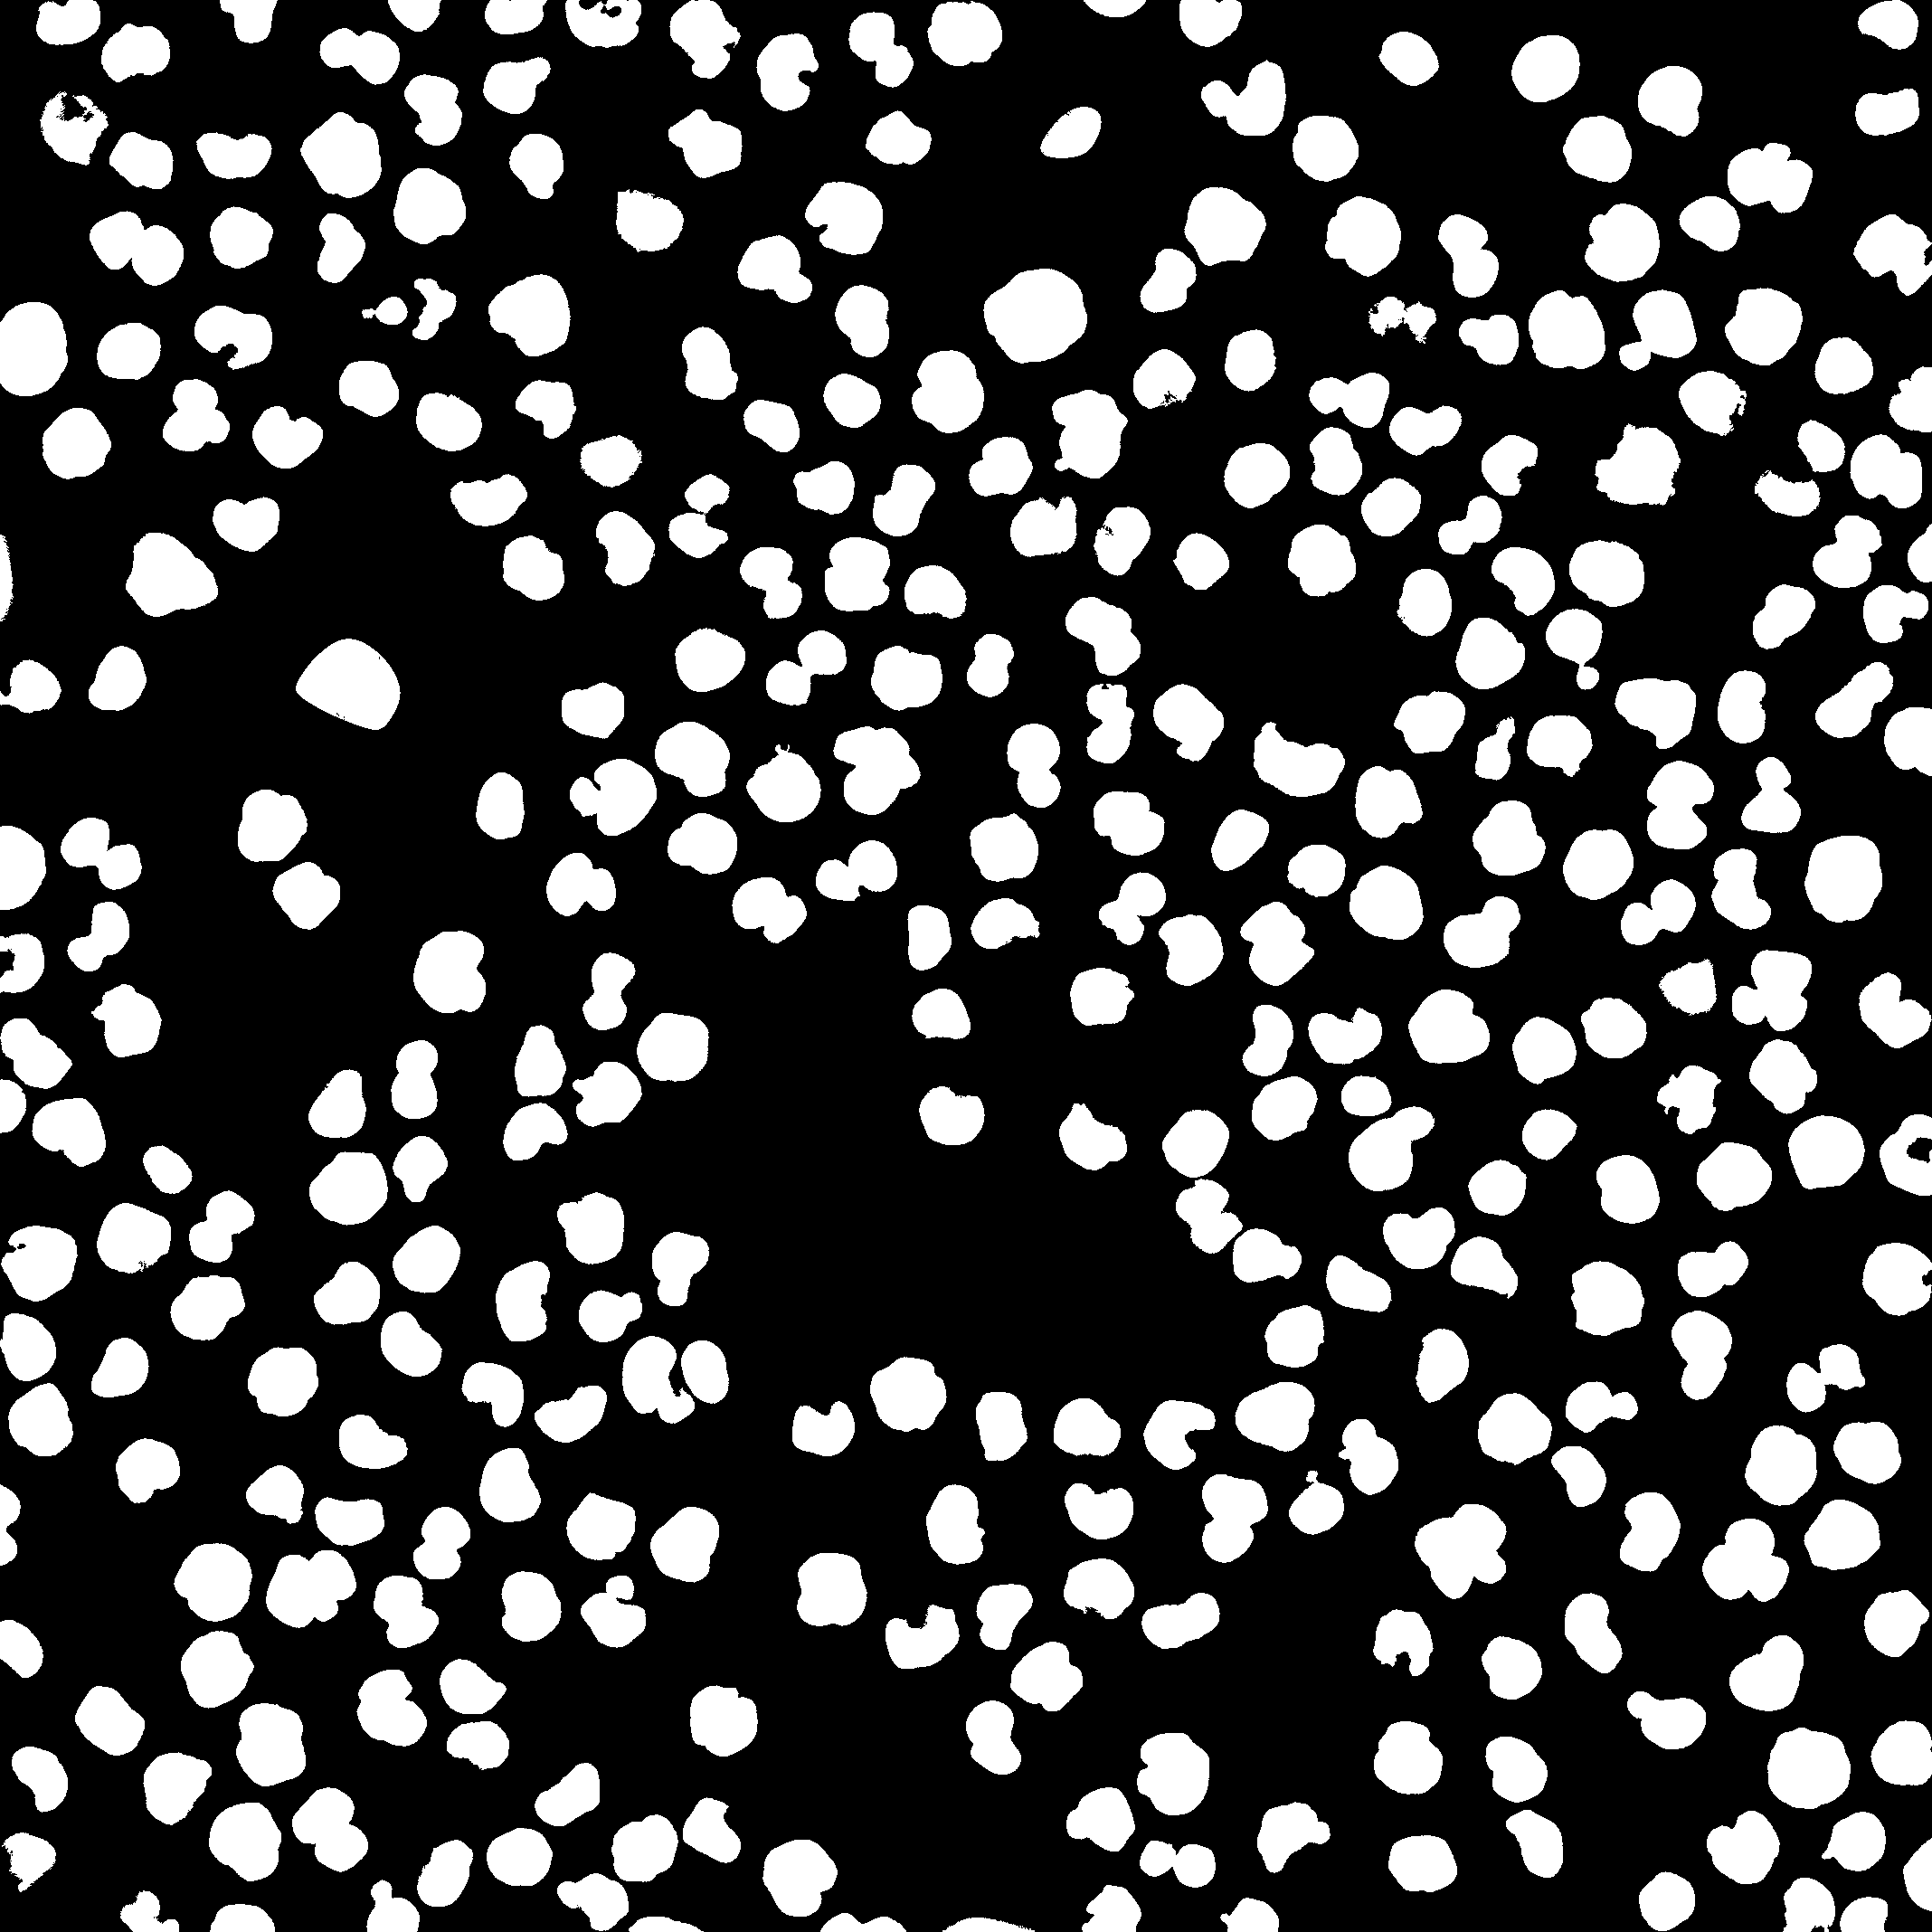
\includegraphics{bilder/segmentation/nuclei-mask/mask.png}
        \end{tabularx}
    \caption{Fluorescence segmentation}
    \label{fig:segmentation-nuclei-steps}
\end{figure}